\documentclass[10pt,twocolumn,letterpaper]{article}
\usepackage[margin=2.5cm]{geometry}
\usepackage{times,epsfig,graphicx,amsmath,amssymb}
\usepackage[breaklinks=true,colorlinks=true,bookmarks=false]{hyperref}
\usepackage{mathtools}
\usepackage{amsmath,graphicx}
%\graphicspath{{code/outputs/}}
\date{}

%%%%%%%%%%%%%%%%

\title{Optical Line Following For Quadcopter UAV}

\author{%
Chris Bonney\\
{\tt bonney@wustl.edu}
}


\begin{document}
	\maketitle
	
%	Right out roughly a one paragraph abstract that introduces your
%	report and project and provides a short summary. Keep this to less
%	than 15 lines.
	\begin{center}\textbf{Abstract}\\~\\\parbox{0.475\textwidth}{\em
			% Abstract goes here
			In this paper I dicuss and simulate an algorithm and controller for a quadcopter UAV drone following a marked path along the ground. The model uses a fast inner-loop controller to control the states of the UAV and a slow outer-loop controller to define the commands. The outer-loop controller uses the output of a Hough Transform to calculate a desired change in orrientation and position, as well as a constant forward velocity. In the simulation, I used a function to approximate output of the Hough Transform by feeding the model the distance and angle to the path with a delay to model the computation time. 
			
	}\end{center}

	\section{Introduction}
	
	Control of autonomous unmanned aerial vehicles (UAVs) is an ongoing field of research. One reason they are important is because they allow professionals and hobbyists alike to gain an aerial perspective or an onsite observer in difficult to reach or dangerous locations at a cheap price. Right now, uses range from monitoring power plants, remote sensing, aerial mapping of crops, to patrolling operations and many more \cite{ceppi}.  Most UAVs are not autonomous and require a human operator, but with autonomy the number of uses for UAVs will soar. 
	
	To solve the simplified autonomous case of optical line following, we need a computer vision algorithm that can take an input image and identify lines in the image, and return properties of the line that can be used to command the UAV. A common algorithm to do this is the Hough Transform, which can be used to not only identify one dominant line, but any number of them. Additionally, the Hough Transform defines lines by their distance and angle relative to the UAV, which are the two parameters that we want to use to control the UAV. 
	
	For this project, I used a non-linear model of the UAV dynamics that I had previously built with Ethan Cuka and Clay Whipp under the guidance of Dr. Sankalp Bhan of WUSTL, and designed a controller to fit this purpose. A block diagram of the system is shown in Figure \ref{fig:block_model}. A limitation of this model and the simulations I did in it is that they do not model the inherently noisy sensor measurements and line uncertainty in line detection. 
	
	To make a successful line follower, we need the individual components of the system, an accurate line detector, and the controller. 
	
	The line detector requirement is more difficult than at first glance: a target line on the ground, like a strip of tape, is not one-dimensional, but the detector should be able to find the center of the strip; the target line may not be straight, and the detector needs to either find a reasonable linearized approximation of the line, or be able to accurately model the curve; a target may also have sharp corners, like right angles that need to be dealt with; fourth, it needs to be computationally fast so that the UAV can update its commands quickly, as well as so that it doesn't use processing power required by the flight controller; lastly, there may be noise or secondary lines in the image that need to be filtered out to find the target line. The CV algorithm I propose mets the first three requirements for an accurate line detector, but does not consider the last. 
	
	Next, we need a controller that uses the commands generated by the line detector to control the UAV. The requirements for this are that the error in the distance and angle to the line are regulated to 0, there is a forward velocity to move along the line, and a constant altitude. The commands for this requirement are shown in Figure \ref{fig:line_cmd}. Because I only considered simulation in this paper, I did not worry about creating an observer for feedback of noisy measurements from the sensors, I assumed the sensors perfectly feedback the actual states. This assumption means that the results are better in simulation than they would be physically. However, since a well-built observer approximates states well, even for noisy sensor data, this assumption is valid to use. 
	
%	\begin{itemize}
%		\item Why is this important?
%		\item What is the CV task?
%		\item Prelude to the rest of the report
%	\end{itemize}
%	
%	Please follow the steps outlined below when submitting your report.
%	
%	\begin{itemize}
%		
%		\item Use either single column figures like \ref{fig:onecol}, or two
%		column ones like \ref{fig:twocol}. Use the [!t] option in latex to
%		make sure all figures are at the top of the page. Add captions to
%		all your figures.
%		
%		\item Try to lay out your report so that the abstract and figure
%		captions tell an ``elevator pitch'' version of your story.
%			\end{itemize}
	
	\begin{figure}[!t] % BLOCK MODEL
		\begin{center}
%			\fbox{\rule{0pt}{3in} \rule{0.9\linewidth}{0pt}} % Place holder, replace with \includegraphics, etc.
		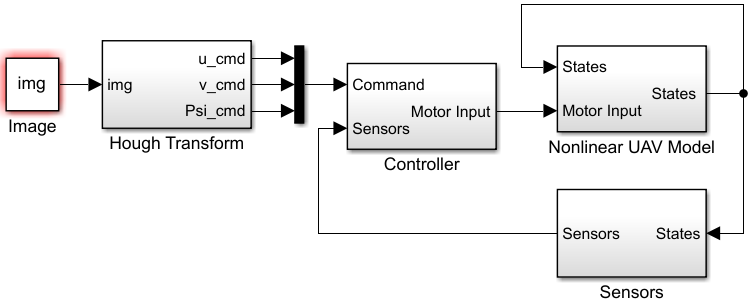
\includegraphics[width=\linewidth]{matlab/block_model}
		\end{center}
		\caption{Block Diagram of Model}
		\label{fig:block_model}
	\end{figure}
	
%	\begin{figure*}[!t]
%		\begin{center}
%			\fbox{\rule{0pt}{4in} \rule{0.9\linewidth}{0pt}} % Place holder, replace with \includegraphics, etc.
%		\end{center}
%		\caption{Example of caption.}
%		\label{fig:onecol}
%	\end{figure*}
	
		\begin{figure}[!t] %COMMAND FROM A LINE
		\begin{center}
			%			\fbox{\rule{0pt}{3in} \rule{0.9\linewidth}{0pt}} % Place holder, replace with \includegraphics, etc.
			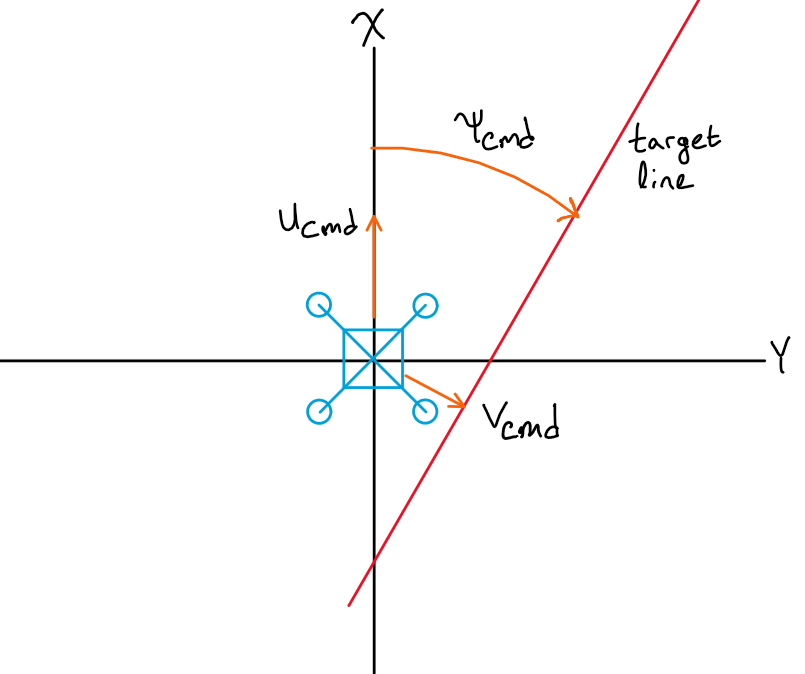
\includegraphics[width=\linewidth]{matlab/controller_model}
		\end{center}
		\caption{Command Inputs from Hough Transform}
		\label{fig:line_cmd}
	\end{figure}
	
	\section{Background \& Related Work}
		In this paper I am exploring a relatively simple form of autonomy: optical line following. There are three common forms of line followers. The first is has been in around for decades and is a common toy, but of very limited use; they are consist of wheeled robots that strictly follow a track by keeping the target, such as a black line, between two sensors, like in this tutorial \cite{arduino}. The second, optical line following, has much broader applications, and is the one I will be discussing in this paper. 
		
		This method takes in an image and finds the most prominent line, and follows it. This second method is what this paper will discuss. Possible applications of this could be a UAV following a highway to track traffic and watch for driving infractions, following a river with a set of sensors for data collection and more. The last one, involves tracking a GPS signal, which has more applications, but also comes with the limitation that the UAV needs to be in constant contact with a GPS satellite which requires a much larger and more expensive drone. 
	
		Every implementation I found of optical line following, by both hobbyists and professionals alike, used a form of the Hough Transform to identify dominant lines in the image, however control methods differed, both in how select a line to follow and in designing a controller to do so \cite{ceppi}\cite{boudjit}\cite{prayitno}. 
		
		The Hough Transform defines lines in an image based on their distance from the center, $r$, and the angle of their normal vector, $\theta$, 
		
		\begin{flalign} 
			r = x \cos(\theta) + y \sin(\theta) \label{eq:hough}
		\end{flalign}
		with $\theta = 0$ describing a vertical line
		
		In his paper, Paolo Ceppi used a controller that had two separate parts, the first to guide the UAV to hover on top of the target line, and the second to guide the drone forward once it was stable above the line, and an input to the Hough Transform as pixels above a certain threshold of color, rather than edges \cite{ceppi}. 
	
		Most implementations used a downward-facing camera for line detection, but Prayinto et al. used a drone with a forward-facing camera for their version, but only in a lab environment \cite{prayitno}. 

		The model and inner-loop controller for the UAV is derived by solving the equations of motion shown below in equation \ref{eq:eq_motion}:

		\begin{flalign} % EQNS OF MOTION
			\begin{split}
				m\dot V + \omega \times mV &= \Vec{F}_G (\phi,\theta,\psi) + \Vec{F}_T \\
				J\dot \omega + \omega \times J\omega &= \Vec{M}_T + \Vec{M}_{gyro} \\
				\dot \phi &= p + \tan\theta (q \sin \phi + r \cos \phi) \\
				\dot \theta &= q \cos \phi - r \sin \phi \\
				\dot \psi &= \dfrac{q \sin \phi + r \cos\ phi}{\cos \theta} \\
				\begin{bmatrix}
					\dot X_{NED} \\
					\dot Y_{NED} \\
					\dot Z_{NED} \\
				\end{bmatrix} &= R^T(\psi)R^T(\theta)R^T(\phi) \begin{bmatrix}
					u \\
					v \\
					w \\
				\end{bmatrix}
			\end{split}\label{eq:eq_motion}
		\end{flalign}

		The system as 12 states: 3 for both its linear positions and velocities, and 3 for the Euler angles and their angular velocities. 
		
		For the purpose of this paper the relevant states are the $X$ and $Y$ velocities, $u$ and $v$, and the $Z$-axis angle or orientation angle, $\psi$. These are the three states that need to be controlled for the line following algorithm. Conveniently, these states are all controlled separately in the traditional Thrust, Elevator, Aileron, Rudder (TEAR) control design, and the fourth control input, Thrust, is used to control the altitude of the UAV.  
		

	\section{Proposed Approach}

	My proposed approach is to design an inner-loop controller using robust-servo Linear Quadratic Regulator (LQR) optimal control to satisfy the regulator requirement, and an outer-loop controller from a variation of the Hough Transform to supply the commands. Since the outer-loop controller doesn't affect critical functions, such as stability, the fact that the Hough Transform takes a relatively long time to compute will not be an issue for the system. 
	
	Other implementations have used Proportional Integral Derivative (PID) controllers for their systems, which are supplied with arbitrary parameters that do not guarantee stability or robustness. Using robust-servo LQR to define the inner-loop controller gives large gain and phase margins to the controller, allowing it to remain stable if given a noisy signal \cite{wise}. 
	
	In his implementation, Ceppi used an intensity threshold to identify valid pixels a Hough Transform, which not only introduces variance in the result by making a range possible lines be identified as dominant, it also takes far more computation time. I propose using a thresholded edge-detection first, and computing the Hough Transform on this. This requires two convolutions of the image to calculate its gradient using sobel derivatives, which costs the majority of the computation time, but results in a much quicker Hough Transform. 
	
	In my approach, I wanted to minimize the computation time of both the Hough Transform, and the edge detection step. The most obvious step was to minimize the size of the image. To do this, I tested naive down-sampling of the image by removing all but every $n$th pixel, to see where accuracy started to be lost. Next, I used the fact that the Hough Transform can identify a number of dominant lines in an image to test for how many should be used to produce the best result.
	
	For the purpose of simulation, I assumed that the UAV could identify the correct line from a ``Virtual Hough Transform'' but at a delay to model the computation time of the operation. I used the average computation time the line detection of a downsized image on my laptop multiplied by 100 as an estimate of the computation time the operation would take on the UAV with much less computation power. This multiplier of 100 is arbitrary, however I don't believe it to be significant, since the simulation had similar performance with and without the delay. 
	
	\section{Experimental Results}
	
	For line detection, I started with a set of images of green tape on a white background. To improve contrast for edge detection, I only considered the green channel. I started by downsizing the image until I reached a point where edges were more noisy than defined. This occurred with images downsized below 50$\times$50 pixels. The accuracy of edges for different downsizes is shown in Figure \ref{fig:downsize}. Note that even for the smallest image at 1/64th scaling, there are still two lines. 
		
	\begin{figure}[!t] %DOWNSCALED EDGES
		\begin{center}
			%			\fbox{\rule{0pt}{3in} \rule{0.9\linewidth}{0pt}} % Place holder, replace with \includegraphics, etc.
			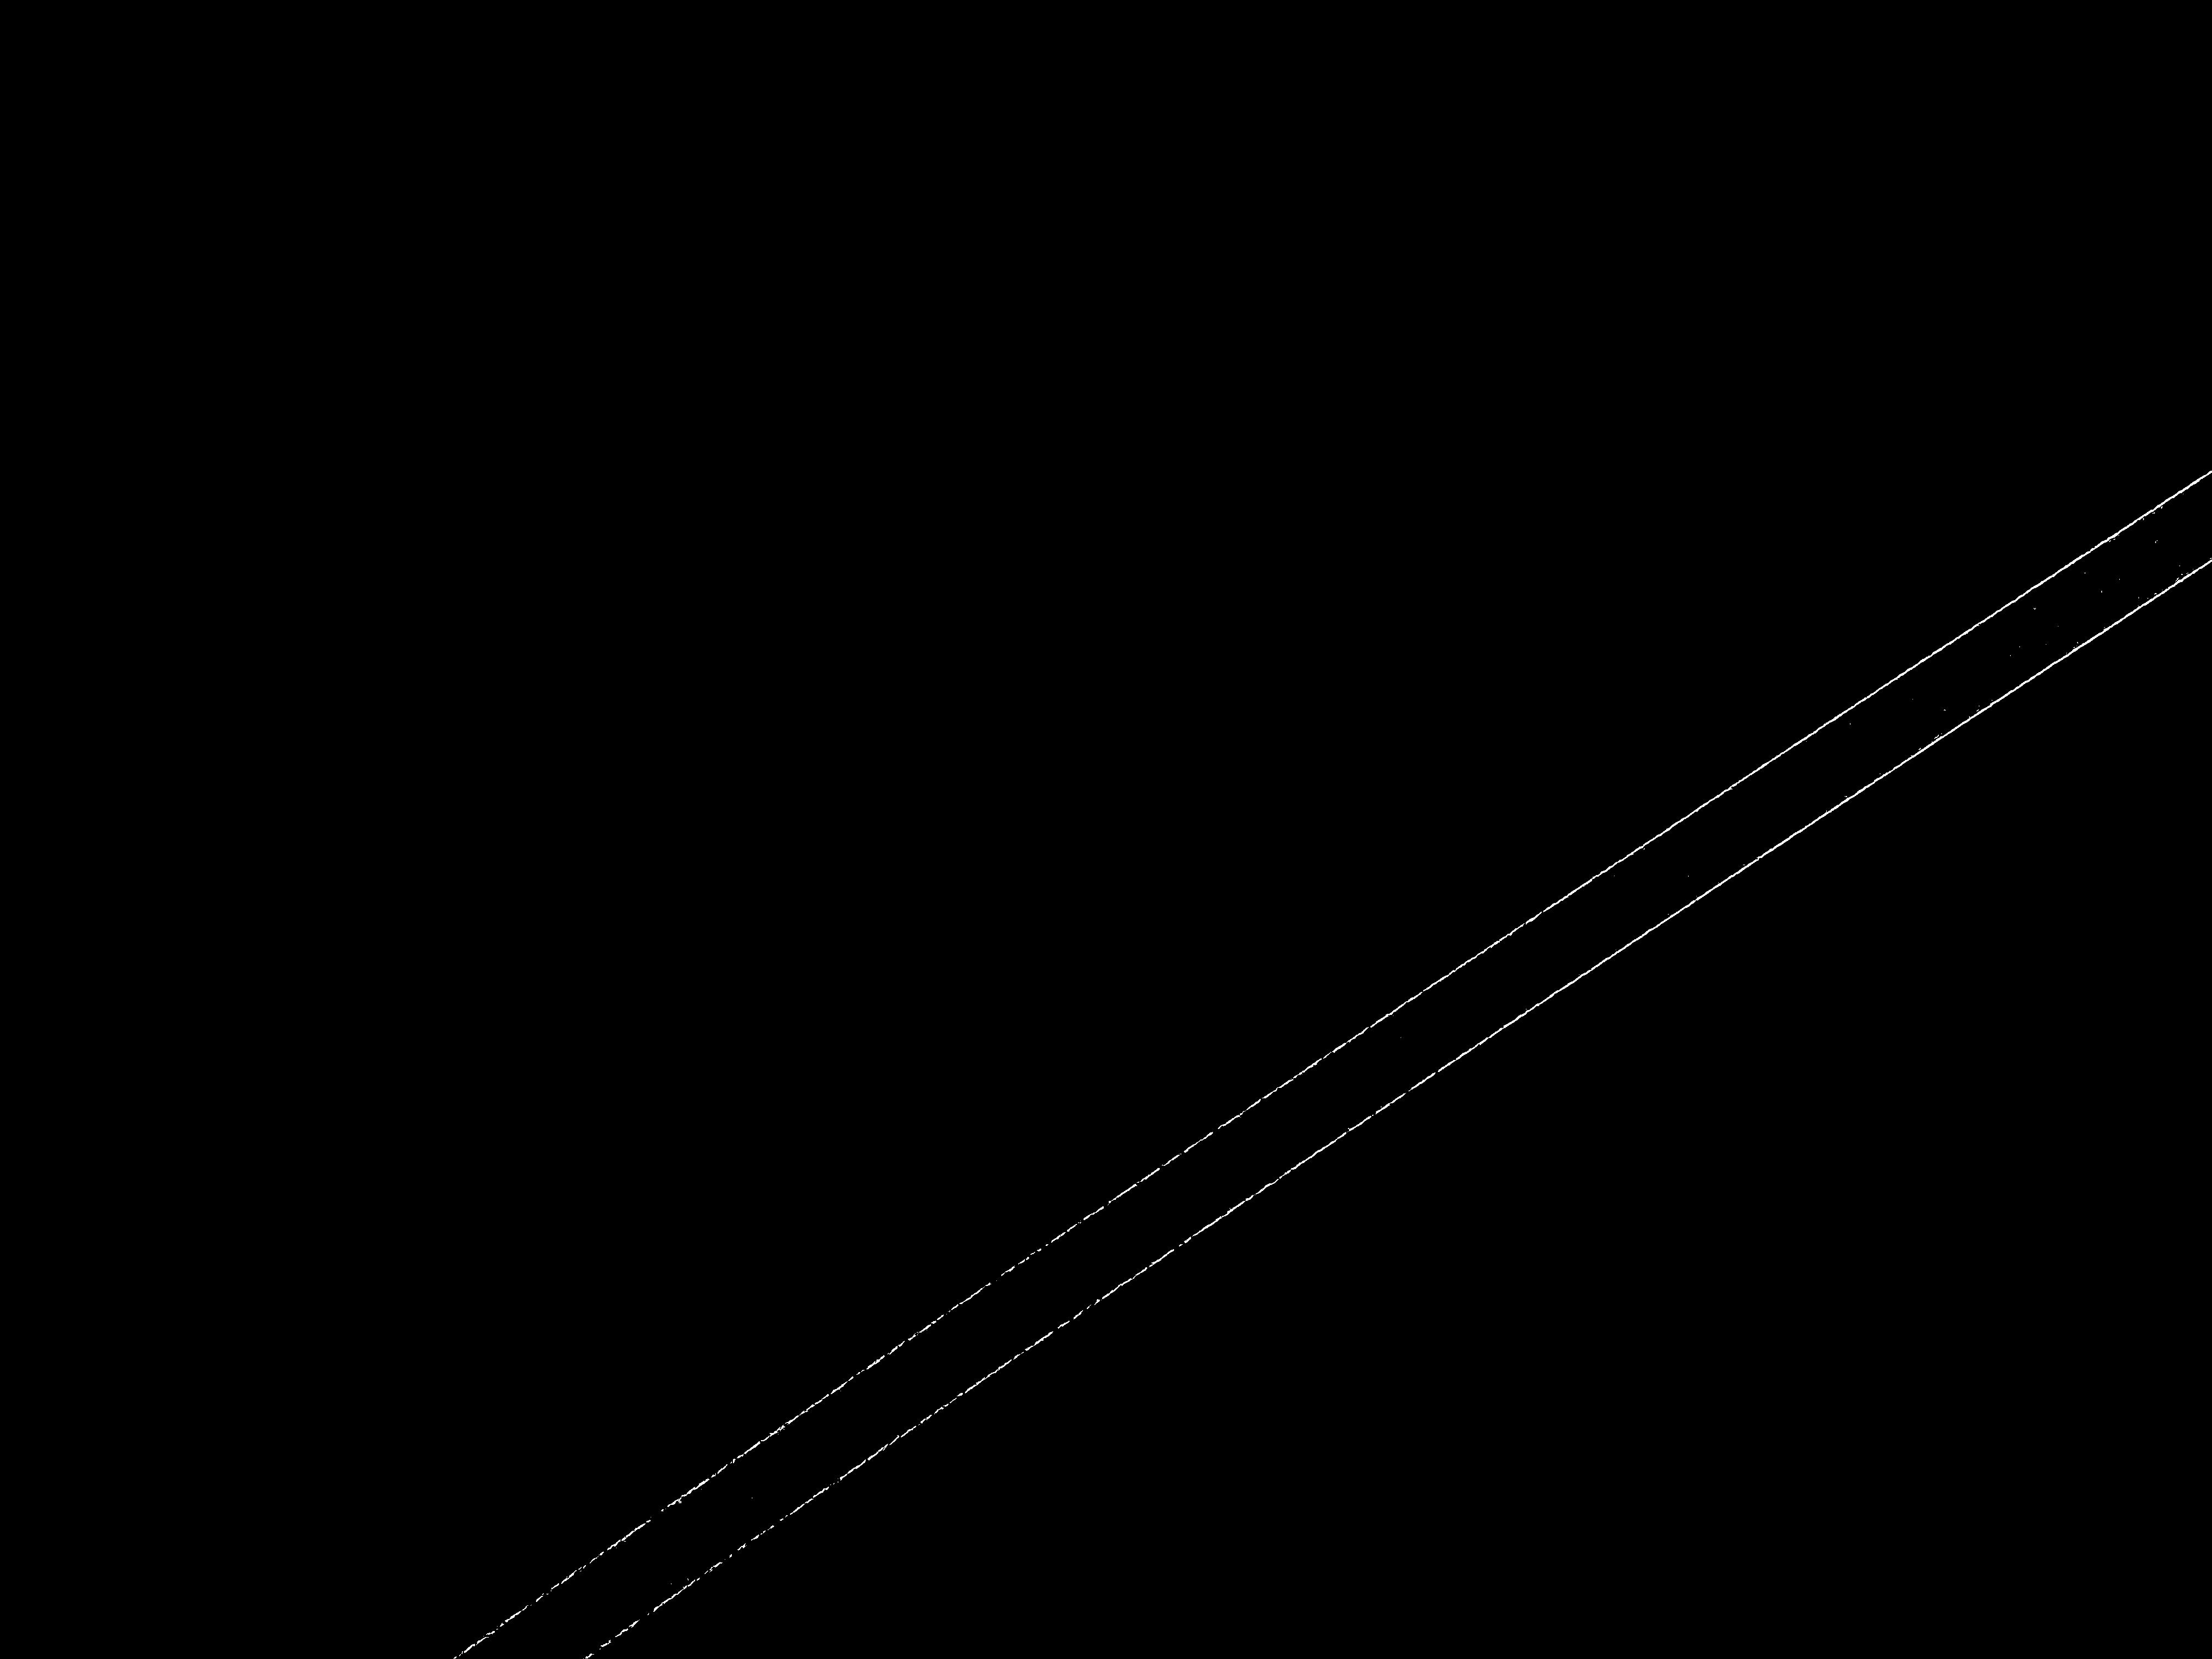
\includegraphics[width=0.6\linewidth]{code/outputs/1_edge_downsize1}
			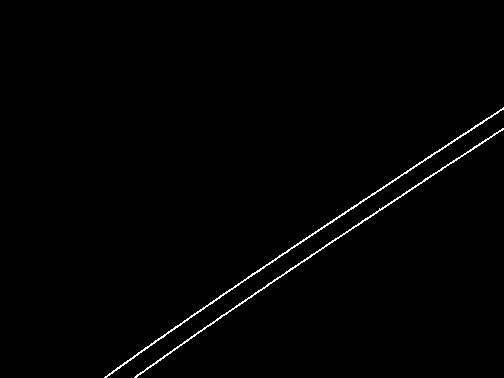
\includegraphics[width=0.6\linewidth]{code/outputs/1_edge_downsize8}
			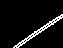
\includegraphics[width=0.6\linewidth]{code/outputs/1_edge_downsize64}
		\end{center}
		\caption{Edges of Downsized Images - top to bottom: 4032$\times$3024 (original), 504$\times$378 (1/8th), 63$\times$48 (1/64th)}
		\label{fig:downsize}
	\end{figure}
	
	After this, I considered whether or not the edges would benefit from Non Maximum Suppression (NMS) before applying the Hough Transform. This could possibly save computation time as well if enough edge pixels were removed. NMS was able to remove on average half the edge pixels of the image. Since the computation time of the Hough Transform is $O(n_p n_\theta)$, where $n_p$ is the number of edge pixels and $n_\theta$ is the number of angles checked for lines in the Hough Transform, this is a significant saving, however it is insignificant compared to the time complexity of the convolutions to calculate the gradient at $O(n_x)$ where $n_x$ is the size of the original image. Additionally, the Hough Transform had worse results since for a low resolution, discretized image some redundancy in edge pixels leads to more confidence in dominant lines. Because of this, I did not use NMS before applying the Hough Transform.
	
	Next I computed the Hough Transform for different types of line to confirm it correctly identified the best line. Because of the thickness of the line, I decided to have the transform return the average of the two dominant lines. In order to make sure it did not detect the exact same line twice, I removed not only the first line from consideration, but every line in a 3$\times$3 grid around it in the transform. 
	
	In theory, this would put the output as the center of the line of tape, however in practice, this only worked for images with straight lines. It did have the side affect of producing a more accurate linearization of a cured line, however, and did not affect images with sharp edges at all. Lastly, I wanted to confirm that for images with sharp edges, the line closest to the center (which defines where the UAV is) will be the dominant line. Intuitively, I expected this to work without any changes to the Hough Transform: the line that is closer to the center will be more contained in the image, and therefore get a larger vote in the Hough Transform. This worked as expected. 
	
	The resulting lines are shown in Figure \ref{fig:detection}. Straight lines are tracked perfectly. Images with curved lines picked a linearization that is almost parallel to the center as desired, and images with sharp edges picked the line closest to the center. 

	\begin{figure}[!t] %LINE DETECTION
		\begin{center}
			%			\fbox{\rule{0pt}{3in} \rule{0.9\linewidth}{0pt}} % Place holder, replace with \includegraphics, etc.
			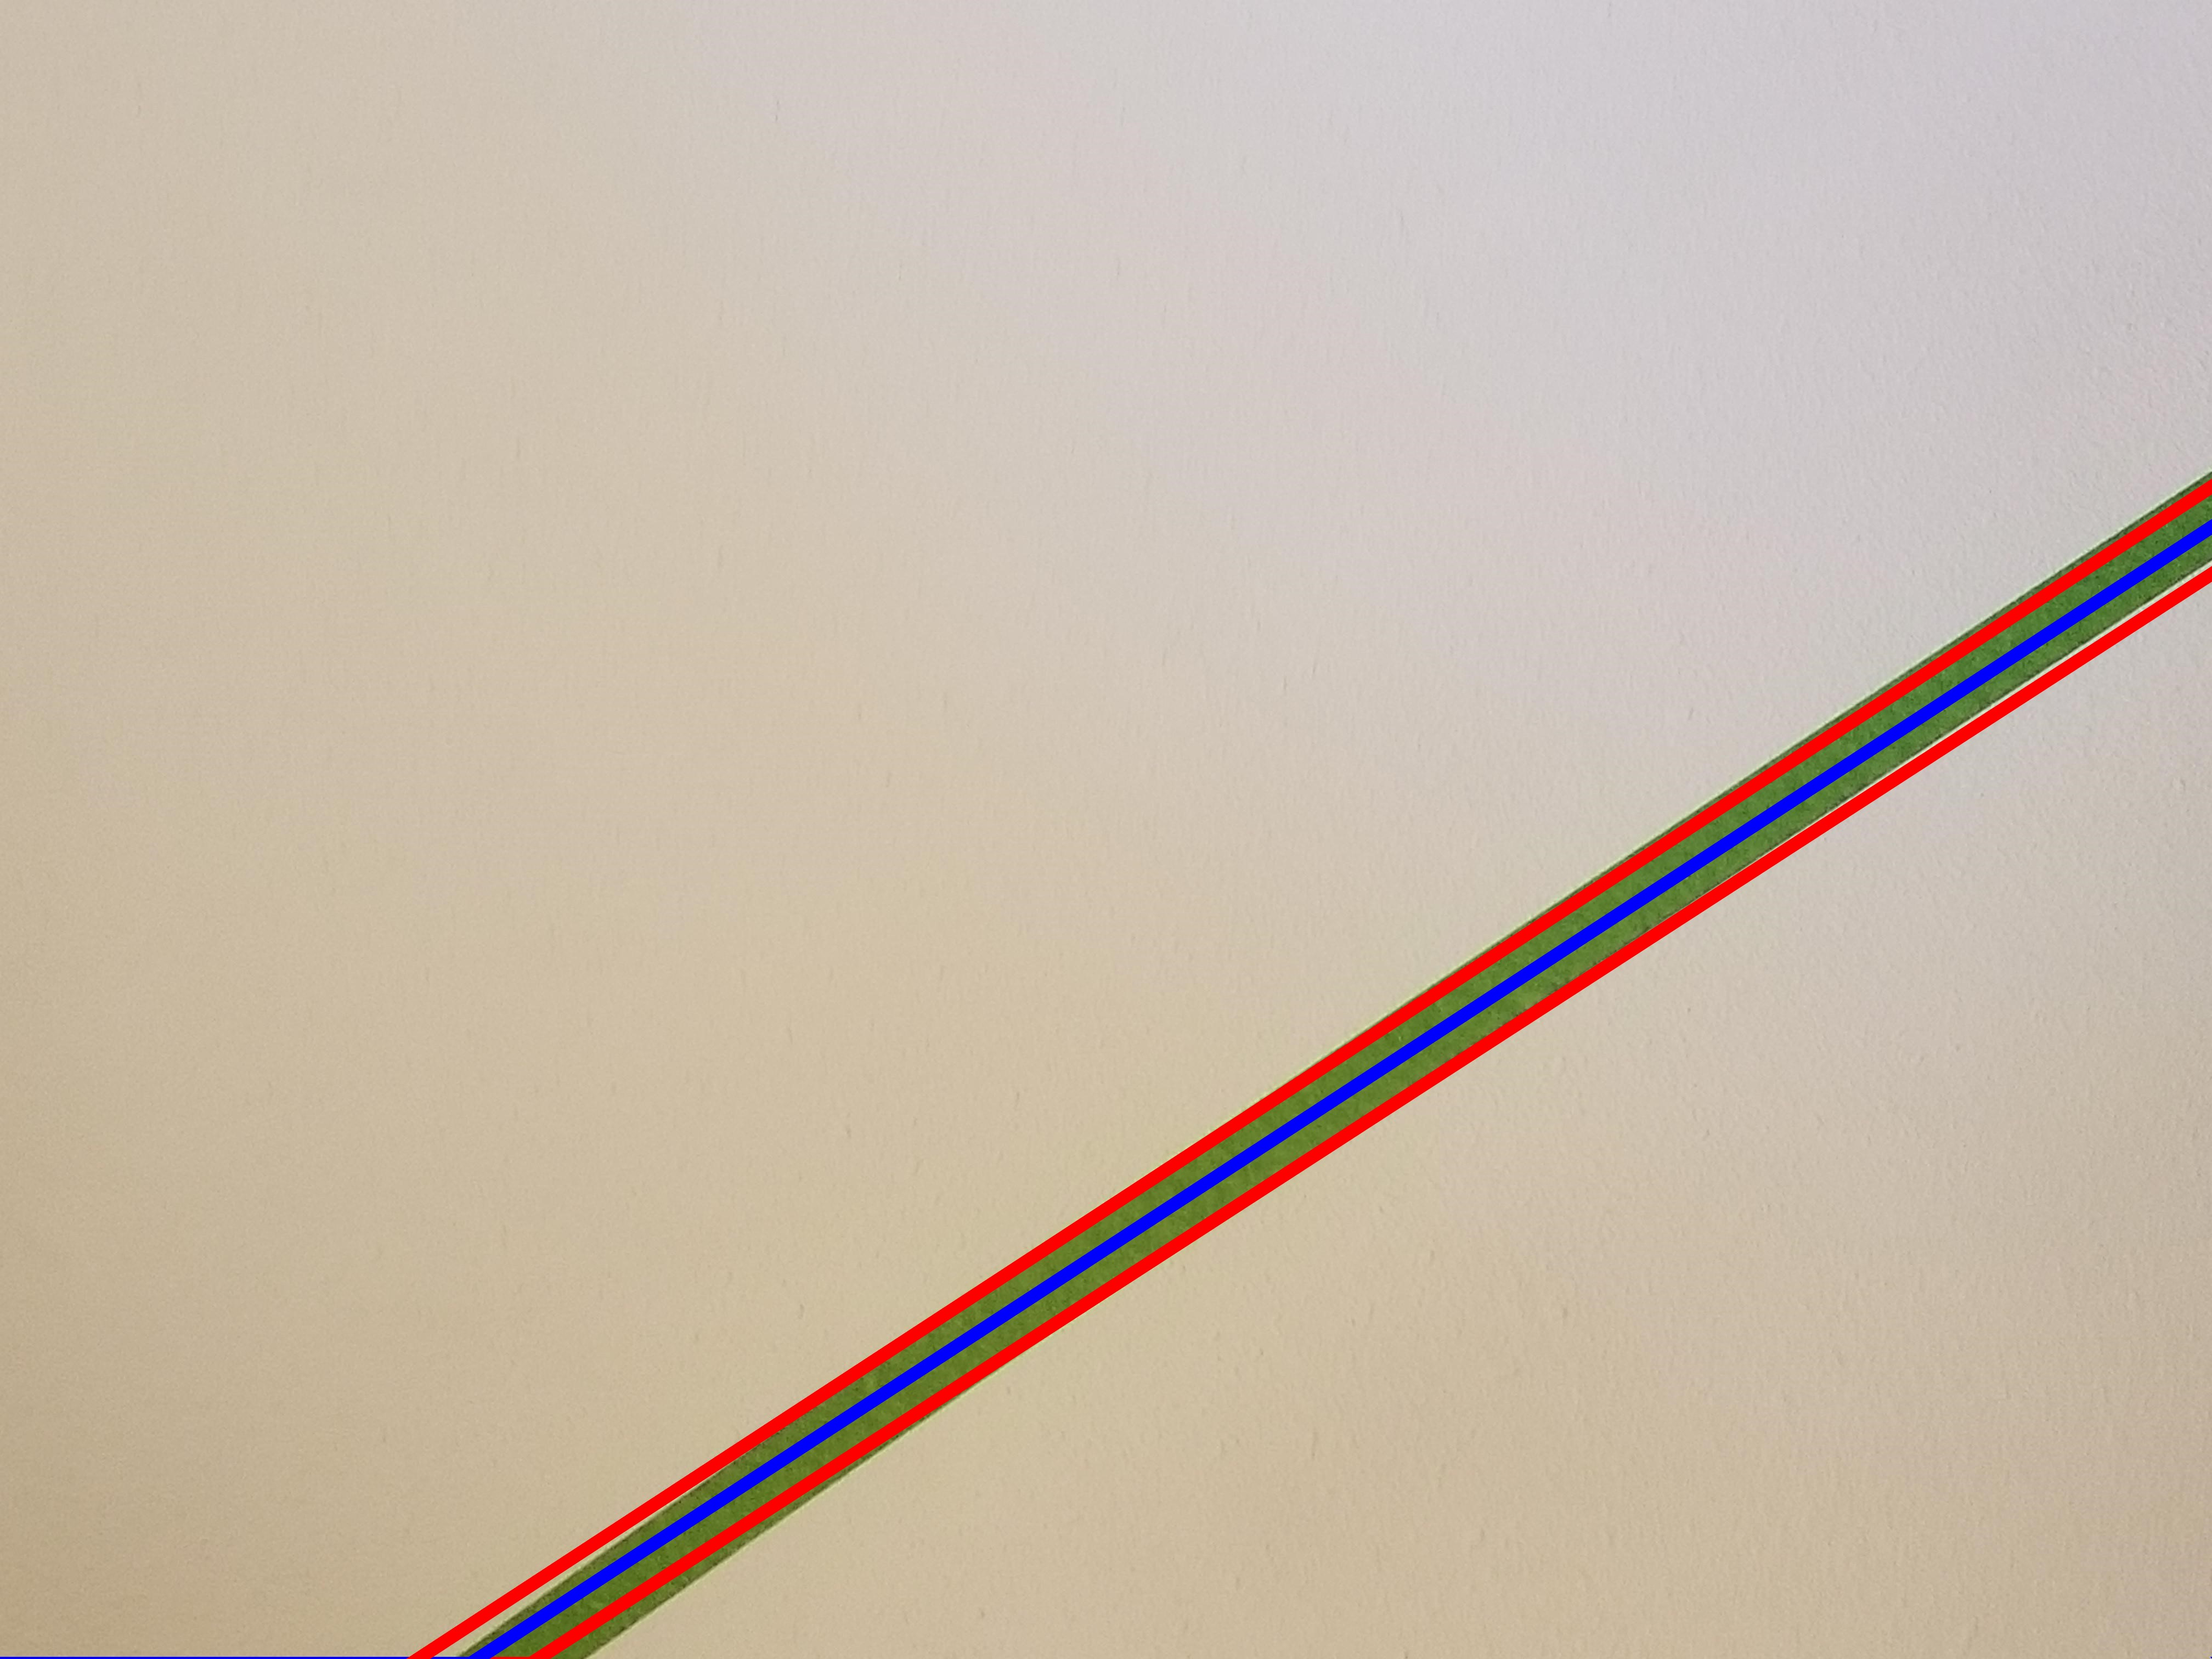
\includegraphics[width=0.7\linewidth]{code/outputs/1_line}
			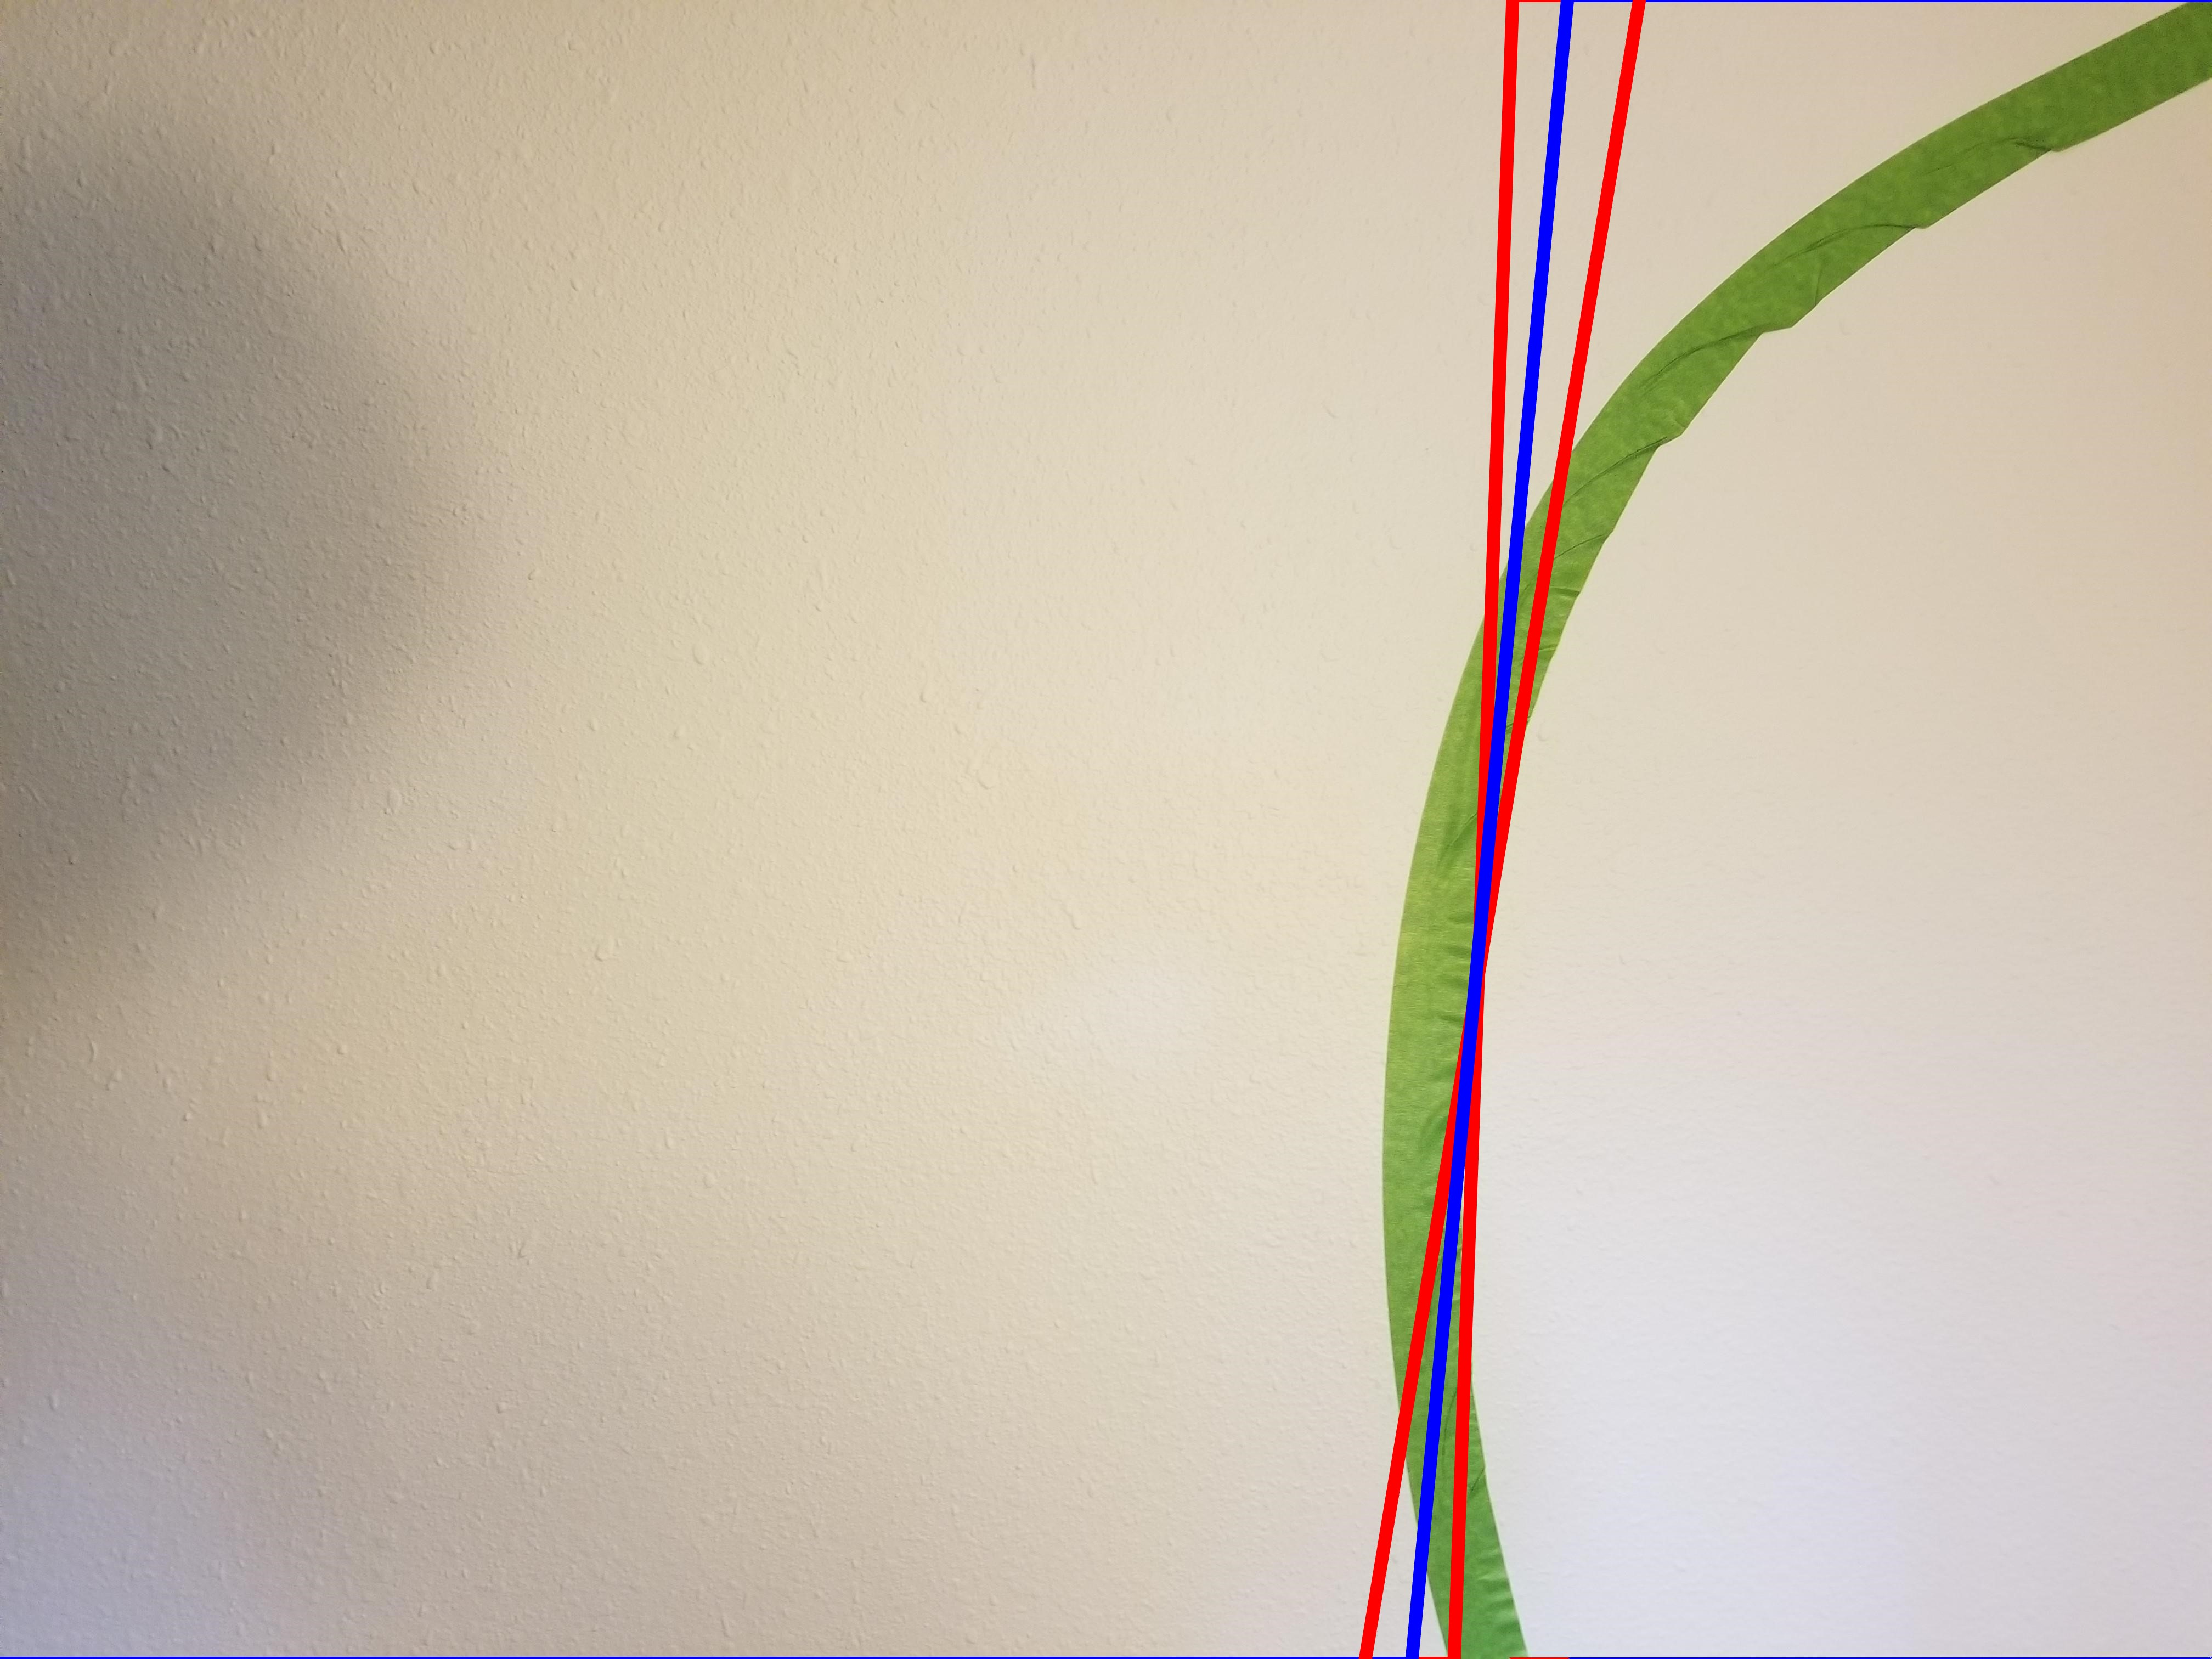
\includegraphics[width=0.7\linewidth]{code/outputs/10_line}
			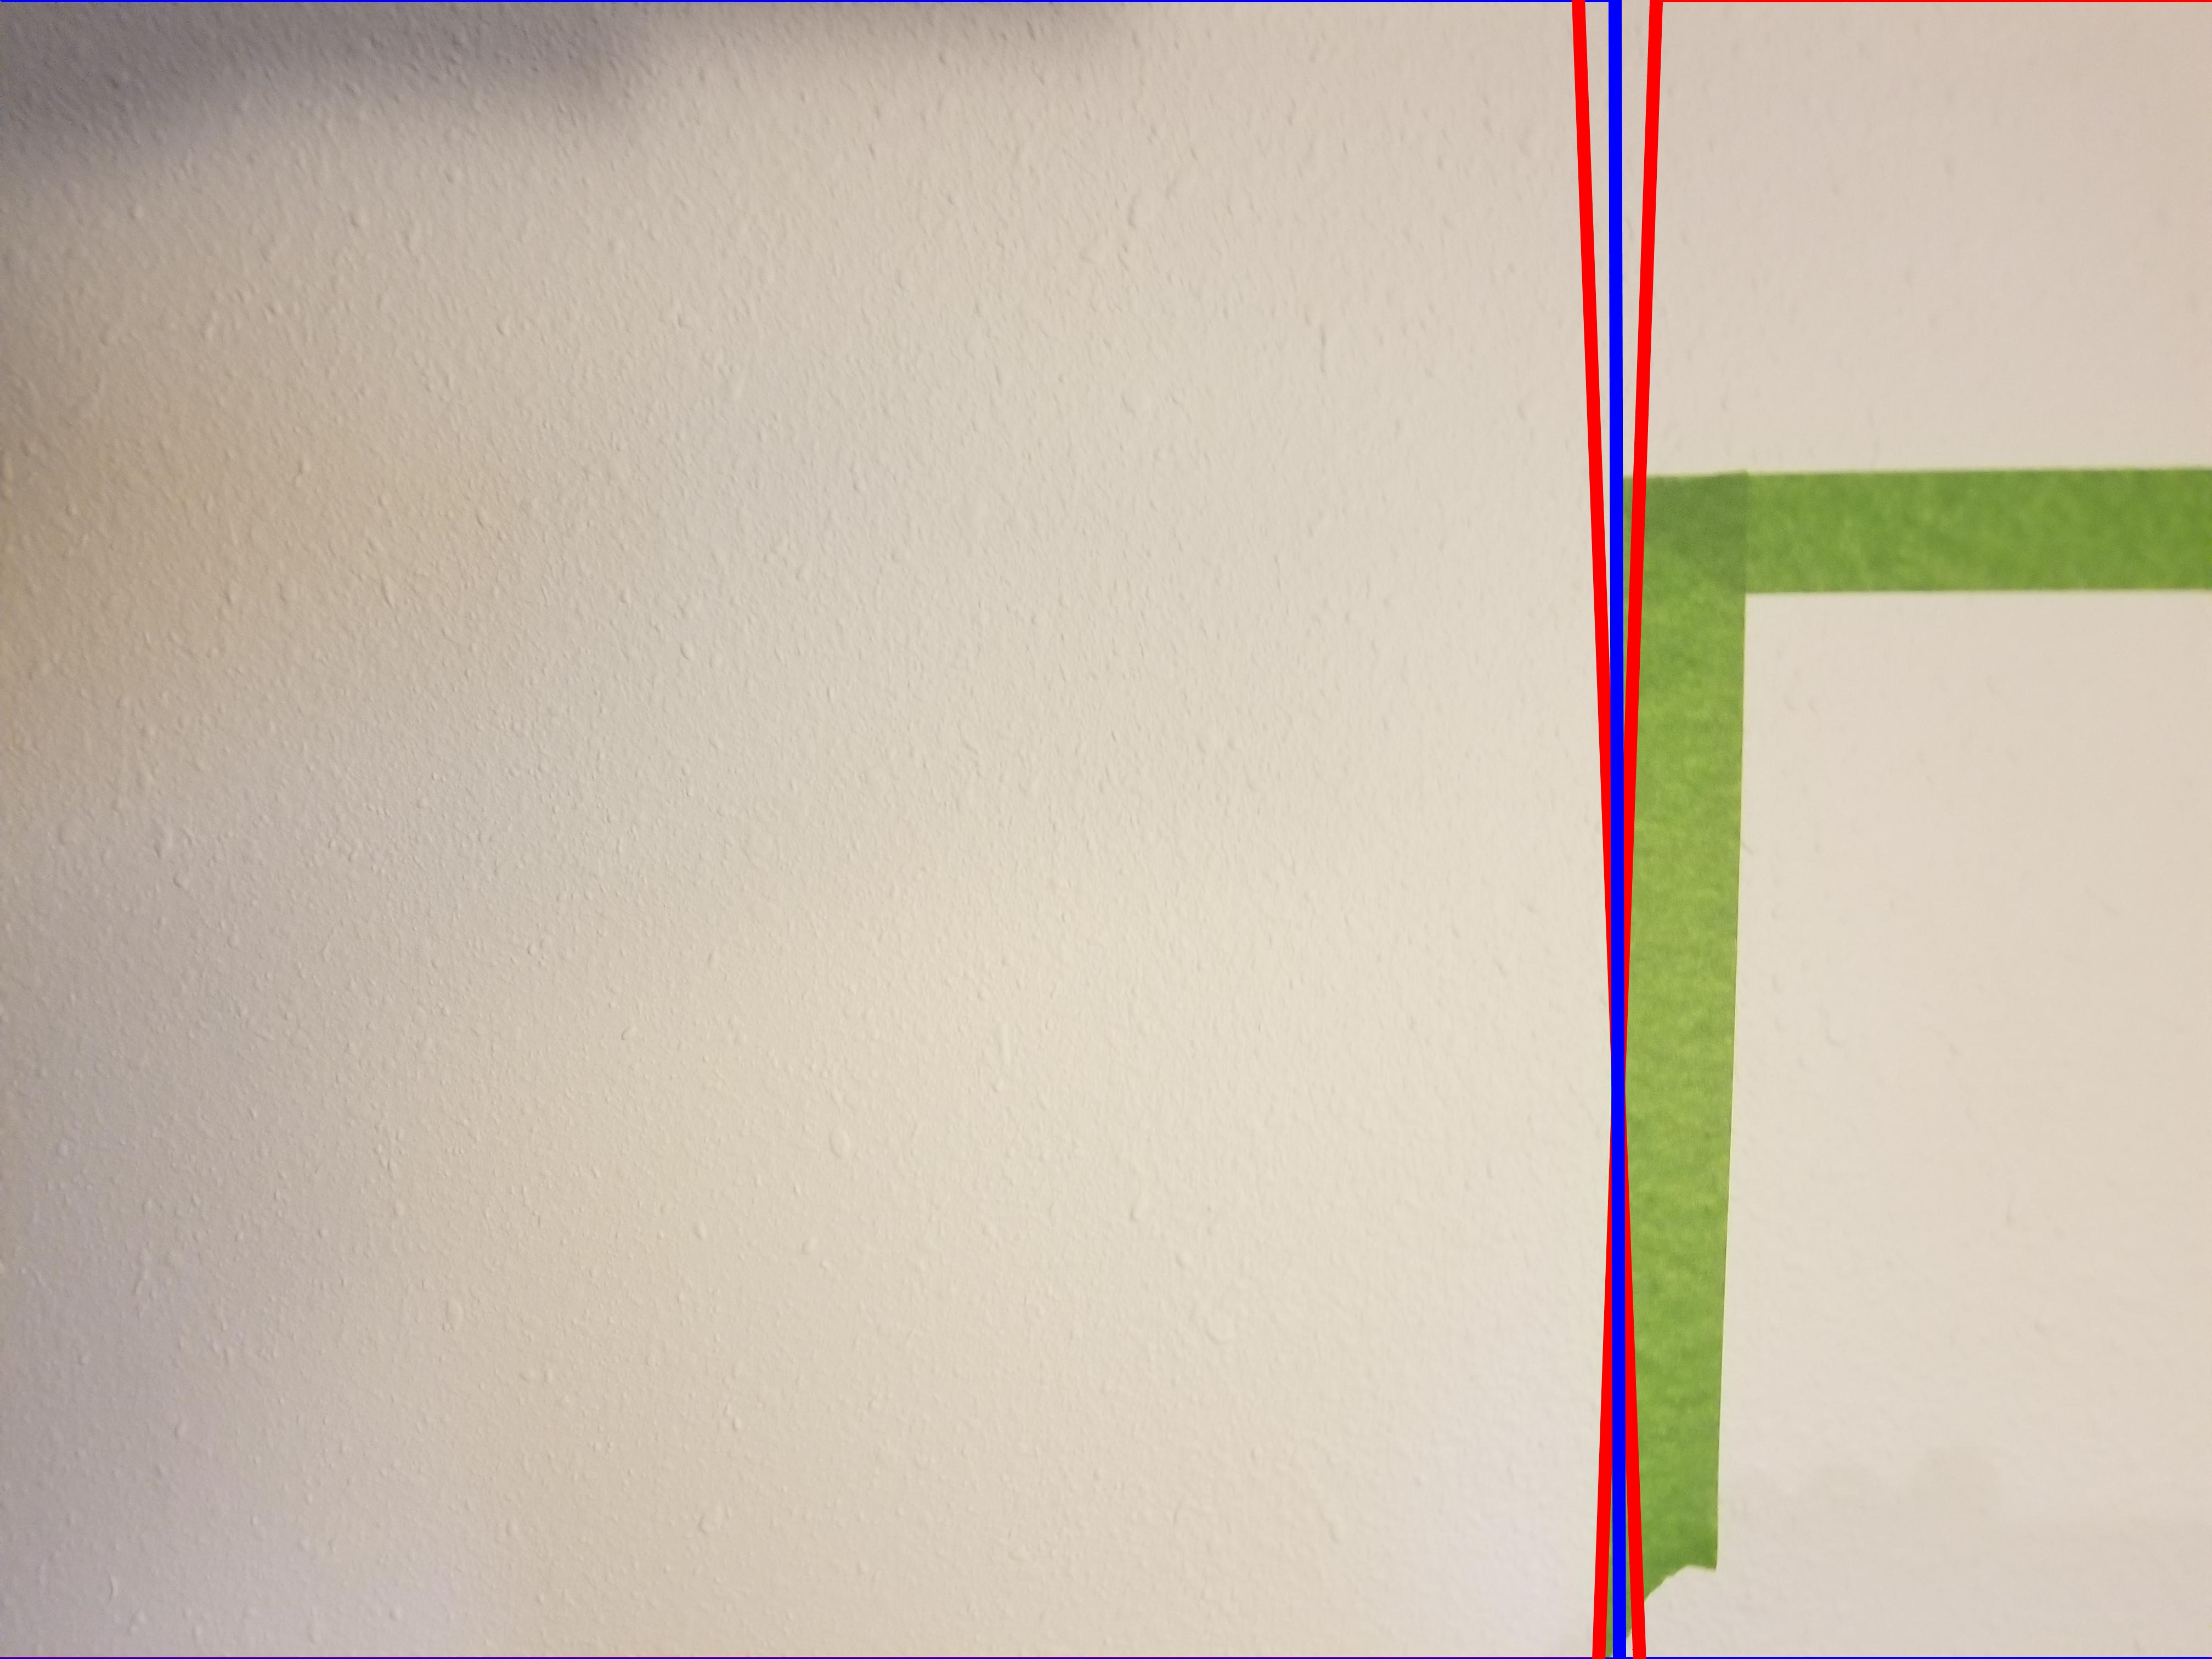
\includegraphics[width=0.7\linewidth]{code/outputs/11_line}
		\end{center}
		\caption{Detected Lines for different shapes. Red are the two most dominant lines, and Blue is their average}
		\label{fig:detection}
	\end{figure}
	
	The average computation time on my computer for an image from downscaling to output was 0.015 seconds. However, a small UAV will have no where near this computing power so it will likely take a much longer time per computation. Because of this, when considering a delay for simulations I multiplied it by 100 to 1.5 seconds computation per image. 

	\begin{figure}[!t] %COMMAND FROM A LINE
		\begin{center}
			%			\fbox{\rule{0pt}{3in} \rule{0.9\linewidth}{0pt}} % Place holder, replace with \includegraphics, etc.
			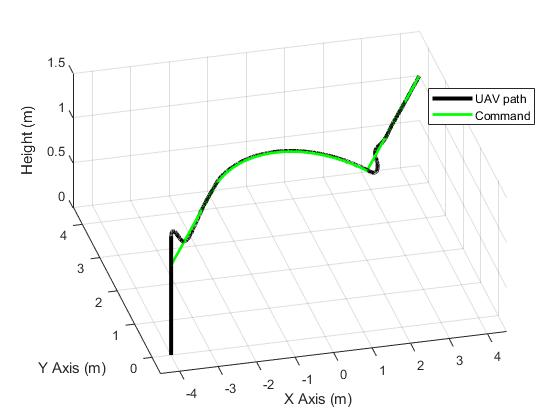
\includegraphics[width=\linewidth]{matlab/combo_path}
		\end{center}
		\caption{Line Follwoing Simulation}
		\label{fig:simulation}
	\end{figure}	

	To simulate the system, I used a Simulink Model following the block diagram shown in Figure \ref{fig:block_model}. To simulate the Hough Transform, since I couldn't use an image, I used output the result of the distance to and angle of the closest line to the UAV at a delay of 1.5 seconds. As we can see in Figure \ref{fig:simulation}, the follower perfectly tracks straight lines and curves, and quickly adjusts to sharp corners of up to $90^o$.

	\section{Conclusion}
	The algorithm and simulation demonstrated in this project, while not robust or applicable on their own, are a strong proof-of-concept for future work such as implementation on the physical drone. There are a number of improvements I would make to the line detection given more time and the knowledge gained from writing this paper, such as attempting to use a smaller window to identify lines when possible to improve accuracy and computation time, and trying to detect a line in front of the UAV to help it predict and handle sharp corners better. 

	\section*{Acknowledgments}
	I would like to acknowledge the two professors whose lectures and materials I leaned upon heavily for this project, but since they are not published, are not listed in the References: Dr. Sankalp Bhan for the creation of the nonlinear dynamics model for the UAV, and Dr. Ayan Chakrabarti for support code I used for image processing and analysis of the Hough Transform. 
	

	
	{\small
		\bibliographystyle{ieee}
		\bibliography{refs} % Create file refs.bib, and run bibtex.
	}
	
\end{document}
